\ch{Implementation}{implementation}

This chapter details the practical realization of the proposed autonomous laboratory framework, translating the conceptual model into a fully operational physical system. Beginning with hardware integration, the implementation progressed through software module development, and agentic orchestration. \textbf{Section~\ref{sec:onhardware}} details the full implementation pipeline, from the creation of the digital twin and assembly of mechanical components to the development of modular Python tools and the deployment of the AI Agent through the \texttt{smolagents} framework. Afterwards \textbf{Section~\ref{sec:tests}} presents simulated validation procedures verifying coordination and reliability prior to live operation. Finally, \textbf{Section~\ref{sec:actualexperiments}} describes user-based evaluations conducted under real laboratory conditions to assess system performance, success rate, and robustness. Together, these sections demonstrate the end-to-end realization of an LLM-driven SDL.

\sect{Real-World Implementation of Modules and Components}{onhardware} 

The implementation process began with the creation of a digital twin of the demonstration environment. This virtual representation replicated the physical layout, instruments, and workflow of the SDL, allowing system development and testing to be conducted in a controlled and risk-free setting. The digital twin provided a consistent framework for verifying motion paths, tool interactions, and communication logic before deployment on the actual hardware, thereby reducing the likelihood of mechanical errors and improving the overall reliability of the integration process.

The physical components required for the demonstration SDL were designed and constructed to match the specifications defined in the digital model. Several custom parts were fabricated using 3D printing, including the sample base and fixture elements, while other components, such as the sample pieces themselves, were precision-cut using CNC machining. This enables the setup to meet the spatial and functional requirements of the experimental workflow.

The hardware configuration used for running the SDL Agent and all associated experiments is summarized below:

\begin{itemize}
    \item \textbf{Processor:} AMD Ryzen 7 PRO 5750G with integrated Radeon Graphics (3.80\,GHz)
    \item \textbf{Graphics:} AMD Radeon(TM) Graphics, 495\,MB dedicated VRAM, 7.86\,GB shared system memory
    \item \textbf{Memory:} 16\,GB DDR4 RAM
    \item \textbf{Operating System:} Windows 11 Enterprise, 64-bit
\end{itemize}

After the hardware components were assembled, the robotic system was integrated into the workstation. The uFactory xArm6 robot was connected via Ethernet using its assigned local IP address, and the official Python API was cloned from the GitHub repository to the project environment. Initial test scripts verified communication, basic motion commands, and workspace accuracy.

The gripper module was then integrated with the robotic arm, and its control routines were implemented using the uFactory Python API to ensure precise, synchronized actuation. Functional testing confirmed stability, and a new home position was calibrated to account for the gripper’s geometry and guarantee collision-free operation.

With calibration complete, the measurement station and user interaction area were positioned to minimize travel distance and maintain an organized workspace. After completing hardware and network integration, the software implementation phase began with the development of modular Python functions representing the SDL’s core experimental operations. Each tool encapsulated a measurement or manipulation task, ensuring interoperability, clarity, and extendability within the autonomous control framework.

As described in Section 3.2, the next stage involved developing the robot’s functional layer until high-level autonomous operations such as pick-and-place were achieved. These functions form the foundation of the SDL’s physical interaction capabilities. Example implementations include measuring a specific sample for a defined electrochemical feature, delivering a selected sample to the user area, or receiving a sample from the user and placing it into a designated slot on the sample base before returning to the home position. Each function was implemented with explicit motion parameters, safety limits, and synchronization routines to ensure deterministic and repeatable execution within the integrated laboratory environment.

To enhance transparency during operation and facilitate debugging, informative print statements were incorporated throughout the mid- and low-level function layers. These messages provide real-time, step-by-step feedback on the system’s current state, executed commands, and process transitions. This continuous information flow allows the user to monitor task progression, verify correct execution, and promptly identify potential anomalies during both development and operation.

Ultimately, the set of software tools developed for the SDL constitutes the functional core of the system. These tools implement the essential laboratory operations and serve as callable units within the agent framework. The tools developed in this work are as follows:

\begin{table}[h!]
\centering
\caption{Overview of Functions in \texttt{tools.py}}
\begin{tabular}{|l|p{10cm}|}
\hline
\textbf{Function} & \textbf{Description} \\ \hline
\texttt{ocp\_measurement(i)} & Automates Open Circuit Potential (OCP) measurement by picking, measuring, and returning the sample. Logs observation with measured value. \\ \hline
\texttt{ca\_measurement(i)} & Performs Chronoamperometry (CA) measurement following the same robotic procedure as OCP. \\ \hline
\texttt{cv\_measurement(i)} & Executes Cyclic Voltammetry (CV) measurement and logs result. \\ \hline
\texttt{bring\_sample\_to\_user(i)} & Transfers a specified sample from its slot to the user interaction area. \\ \hline
\texttt{collect\_sample\_from\_user(i)} & Collects a sample from the user area and returns it to a defined slot. \\ \hline
\texttt{go\_home()} & Moves the robotic arm safely to its home position and logs the state. \\ \hline
\end{tabular}
\end{table}

With the implementation of the core SDL tools completed, the next phase focused on developing the AI Agent responsible for orchestrating these functions. This component serves as the system’s decision-making layer, translating user instructions into structured tool executions within the autonomous laboratory environment.

The AI Agent was implemented using the \texttt{smolagents} framework, which provides a lightweight structure for tool-based language model orchestration. The framework components \texttt{CodeAgent}, \texttt{LiteLLMModel}, \texttt{GradioUI}, and \texttt{tools} were imported to construct the agent's reasoning and interaction pipeline. In addition, the previously developed SDL tools were integrated into the agent's environment, enabling direct access to laboratory functions through structured tool calls initiated by user input.

As described in Section~3.2, the \texttt{Qwen2.5-Instruct} model with 7~billion parameters was selected as the language model for the AI Agent. The model was executed locally using the \texttt{Ollama} backend, which allows efficient on-device inference without reliance on external APIs. Within the implementation, ensuring security and independency. The model can be instantiated as follows:

\begin{lstlisting}[language=Python, caption={LLM Model}]
model = LiteLLMModel(
    model_id="ollama/qwen2.5:7b-instruct",
    api_base="http://localhost:11434",
    system_prompt="You are a robotic lab assistant. Use ONLY the provided tools."
)
\end{lstlisting}

Subsequently, a system prompt was defined to specify the agent's operational scope, including permissible actions, constraints, and tool usage rules with examples. This prompt serves as the primary instruction set guiding the agent's behavior during task execution. The complete version of the prompt used in this implementation is provided in the Appendix.

After defining the system prompt in the way described in Section \ref{sec:methodological}, the next step involved creating the AI Agent instance. During initialization, the model specified earlier (\texttt{LiteLLMModel} with the \texttt{Qwen2.5-Instruct} implementation running on the \texttt{Ollama} backend) was assigned as the agent’s reasoning component. The agent was then provided with access to the previously implemented SDL tools, enabling it to invoke these functions autonomously when required. Finally, the instruction set defined in the system prompt was integrated to establish the operational logic and behavioral constraints of the agent. The resulting configuration can be summarized as follows:

\begin{lstlisting}[language=Python, caption={Creating the Agent}]
agent = CodeAgent(
    model=model,
    tools=[ocp_measurement, ca_measurement, cv_measurement,
           bring_sample_to_user, collect_sample_from_user, go_home],
    instructions=prompt,
    add_base_tools=False
)
\end{lstlisting}

To enable user interaction with the system, a \texttt{GradioUI} instance was launched to provide a convenient and accessible chat-based interface for communicating with the agent. The interface allows users to issue NL instructions and observe the corresponding system responses in real time. The setup was initiated with the following line of code:

\begin{lstlisting}[language=Python, caption={Launching GradioUI for a Chat Interface with a conventional UI}]
GradioUI(agent).launch()
\end{lstlisting}

With these steps completed, the software implementation phase was concluded. At this stage, both the functional SDL tools and the AI Agent were fully integrated, establishing a complete and operational framework for autonomous laboratory control and interaction.



\sect{Simulated Test Cases for Validation}{tests} 

After completing the integration of the system, a series of preliminary test runs were conducted to verify the stability and functionality of the implemented software and hardware components. Since the SDL is designed for electrochemical experiments, performing full liquid-based procedures at this stage would have introduced unnecessary complexity and contamination risks. Therefore, the initial tests focused on validating the backend logic and the coordinated motion of the SDL’s mechanical subsystems, ensuring that all movements and tool interactions operated correctly within the defined workspace before engaging in real experimental procedures.

To enable safe testing without the use of actual electrochemical materials, a set of simulated measurement functions was implemented to emulate the behavior of the potentiostat. These functions produce randomized but physically plausible output values, allowing verification of data flow, logging, and system response without involving real electrochemical reactions. The simulation also facilitates validation of the AI Agent’s reasoning and tool-calling logic under realistic operating conditions. An example implementation of these placeholder measurement functions is shown below:

\begin{lstlisting}[language=Python, caption={Simulated Measurement Functions}]
class instruments:

    @staticmethod
    def ocp_measurement_step():
        v = random.uniform(0, 1)
        print("Open Circuit Potential measurement started...")
        print(f"OCP measurement done. Result: {v:.3f} V")
        return v

    @staticmethod
    def ca_measurement_step():
        v = random.uniform(0, 1)
        print("Chronoamperometry measurement started...")
        print(f"CA measurement done. Result: {v:.3f} A")
        return v

    @staticmethod
    def cv_measurement_step():
        import random
        v = random.uniform(0, 1)
        print("Cyclic Voltammetry measurement started...")
        print(f"CV measurement done. Result: {v:.3f} V")
        return v
\end{lstlisting}

With the software and simulation components fully implemented, the next stage involved testing the performance of the LLM-based AI Agent. The initial tests were conducted to evaluate the system’s response to well-defined input queries that align with the full range of available SDL functionalities. A total of fifty queries were formulated to represent typical and boundary-case interactions with the system. The agent was launched through the \texttt{GradioUI} interface, which provided an interactive platform for entering NL commands and observing the corresponding actions and responses in real time.

Following the initial evaluation, an additional set of one hundred queries was created using varied phrasing, sentence structures, and semantic patterns to assess the agent’s generalization capability and robustness to linguistic diversity. To accelerate the validation process and ensure consistent testing conditions, an intermediate software layer was introduced to automate query submission and result collection. This approach enabled the systematic generation of validation data, reduced manual interaction, and facilitated quantitative analysis of the agent’s performance across a larger and more diverse query set.

A dataset of one hundred example queries was composed to evaluate the agent’s ability to interpret diverse NL inputs. Each query represents a potential user instruction formulated with varying syntax, word choice, and structure while referring to the same set of laboratory operations. The dataset includes simple, sequential, and compound instructions involving different samples and measurement types. Example entries from the dataset are shown below:

\begin{lstlisting}[language=Python, caption={Example User Query Dataset}]
{"id": 1, "text": "do ocp for sample 1 then cv for sample 1"}
{"id": 10, "text": "conduct ocp then ca on the 3rd specimen"}
{"id": 26, "text": "measure cv on second and park home"}
{"id": 53, "text": "run ocp for sample three, afterwards bring it"}
{"id": 76, "text": "collect sample 4 from user area and go home"}
{"id": 99, "text": "bring me the third sample and perform all tests ocp ca cv"}
\end{lstlisting}

This dataset served as the primary input source for large-scale validation and performance assessment of the AI Agent.

Subsequently, the agentic execution was initiated using the previously prepared query dataset. For each query, a structured set of performance metrics was collected to enable quantitative evaluation of the system. The recorded data included the execution status (success or failure), total process duration, tracing identifier, and token usage statistics for both input and output. These metrics provided a detailed overview of the agent’s operational reliability, computational efficiency, and resource consumption during interaction with the SDL environment.

A custom tracing system was implemented to uniquely identify each process sequence executed by the agent. The tracing number encodes the sequence of laboratory actions performed during a given query, allowing direct comparison between the intended and executed operations. For example, if the agent performed an OCP measurement on the first sample followed by a CV measurement on the third sample, the corresponding tracing number would be recorded as \texttt{OCP1CV3}. This structure enables precise tracking of multi-step tasks and facilitates validation by linking the agent’s output to the expected experimental sequence defined in the original query.

After completing the developer-led test runs, the next phase involved user-based evaluation to assess the SDL Agent’s performance in realistic interaction scenarios. A group of potential users was invited to operate the system and perform experimental tasks using NL instructions relevant to their intended applications. This stage aimed to evaluate the agent’s usability, interpretability, and robustness when interacting with individuals who were not directly involved in its development, thereby providing a more objective measure of its practical effectiveness.



\sect{User Testings for Validation}{actualexperiments} 

For the user evaluation, five candidates with varying levels of expertise and disciplinary backgrounds participated in the experimental runs. The group consisted of the Head of the Division Material and Surface Technologies at BAM, one postdoctoral researcher in electrochemistry, one doctoral candidate in electrochemistry, one doctoral candidate in computer science and automation engineering, and one master’s student employed as a student assistant. This selection ensured a balanced representation of both domain specialists and technically oriented users, enabling a comprehensive assessment of the SDL Agent’s usability across different professional profiles.

Each participant was individually introduced to the SDL control interface, where direct interaction with the AI Agent was possible. Before commencing the experiments, participants were provided with a two-page briefing document describing the SDL Agent’s capabilities and limitations, the layout of the experimental setup, and the terminology understood by the system. This document, included in the Appendix, ensured that all users had a consistent understanding of the environment and the scope of possible interactions before engaging with the agent. After the introduction, each participant engaged with the agent independently, formulating NL instructions based on their own understanding of the system and observing how the agent executed the corresponding laboratory actions in response.

\begin{figure}[H]
    \centering
    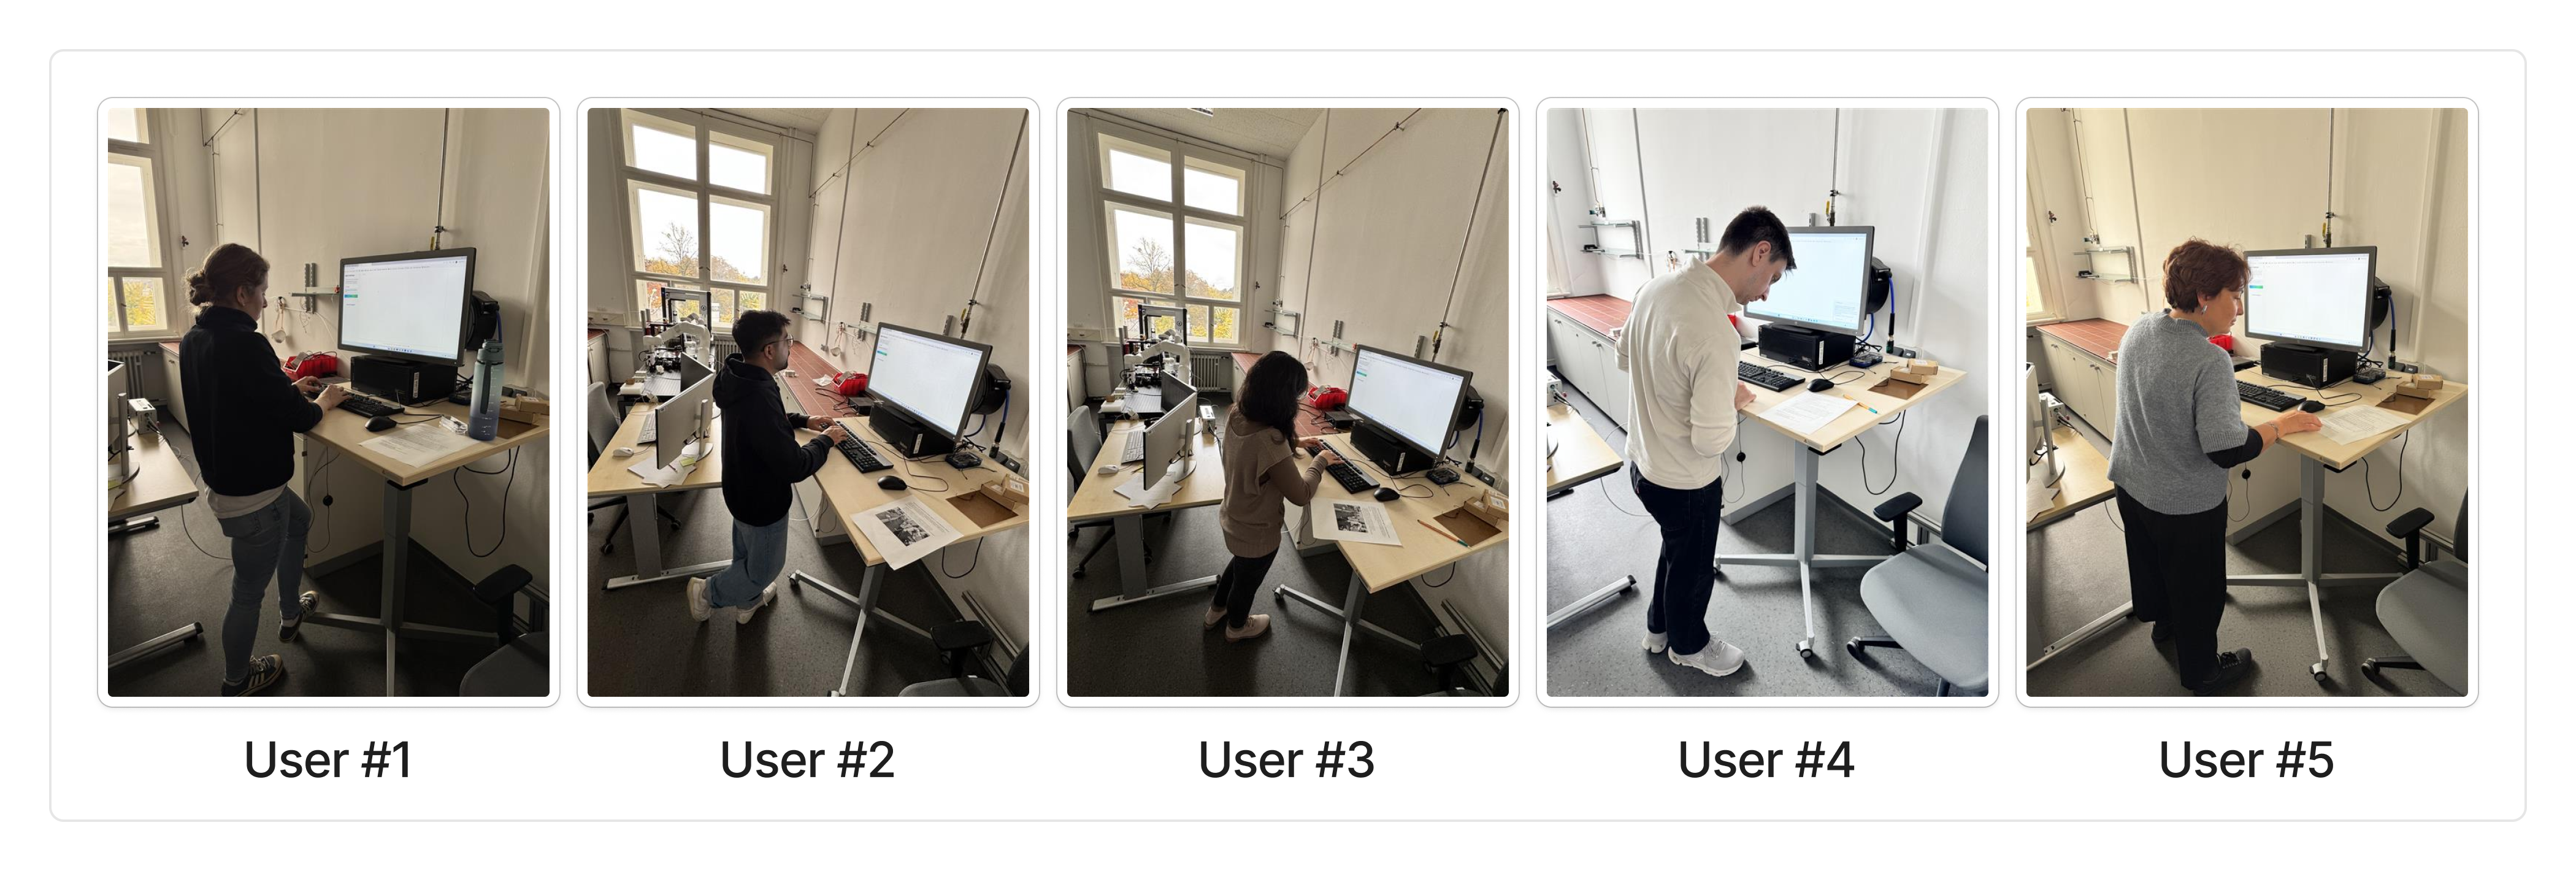
\includegraphics[width=1\linewidth]{Images/users.png}
    \caption{Users conducting experiments in a real lab enviroment}
    \label{fig:users}
\end{figure}

All five participants engaged with the AI agent using distinct linguistic and semantic patterns. Communication styles ranged from formal and conversational to minimal and task-oriented, revealing variations in how users express intent and contextual assumptions. In total, 25 queries were collected, 5 per participant. These inputs captured a broad spectrum of phrasing precision, syntactic structure, and contextual completeness, forming a representative dataset for assessing the agent’s interpretive reliability under authentic user conditions. Example entries from the collected dataset are shown below:


\begin{table}[H]
\centering
\caption{Selected queries from each user}
\begin{tabular}{|l|p{10cm}|}
\hline
\textbf{User No. and index} & \textbf{Query} \\ \hline
\texttt{User \#1, index \#3} & Collect my sample from the user area and place it in the third slot. Then measure an OCP. Return the sample to the user area and collect the next sample and repeat process.\\ \hline
\texttt{User \#2, index \#3} & Put the sample back in the rack for cleaning.\\ \hline
\texttt{User \#3, index \#5} & first measure OCP for 200 seconds, then CV 50 cycles from -0.2 to 0.2 V vs. OCP and then measure CA in one hour with -0.4 V vs. OCP.\\ \hline
\texttt{User \#4, index \#5} & take sample from slot 1 then put it in slot 2 then take it back and put it in slot 3\\ \hline
\texttt{User \#5, index \#2} & Measure for all samples OCP and run for the sample with the highest ocp also CV and then CA.\\ \hline
\end{tabular}
\end{table}

After completing the real-world demonstration experiments with all participants, the collected data were analyzed to assess the overall performance of the SDL Agent. With both simulated and user-driven interaction phases concluded, the study proceeded to the results, focusing on accuracy, success rate, and responsiveness across all tested scenarios.
